\chapter{CloudWatch}\label{ch:cloudwatch}

Amazon CloudWatch is a monitoring and observation tool which can provide developers with insights to monitor
applications, react to performance changes, and optimise resource consumption.
CloudWatch collects monitoring and operational data about the application as logs and metrics to provide a
complete overview of operation health, resource consumption, and the services currently running on AWS\@.
This is useful for any cloud-based application as it allows developers to set alarms, visualise metric logs,
troubleshoot errors and, most importantly, identify and correct anomalous behaviour~\parencite{amazon2022amazon}.
An example of CloudWatch usage would be an alarm set to alert developers when a specified resource consumption level
is over a certain threshold.

For the purposes of the project, multiple CloudWatch alarms will be set up which will allow monitoring for budgeting
and performance across the various AWS services used.

The first alarm which will be set up is a network alarm.
Through selecting the \mintinline{zsh}|NetworkPacketsOut| metric on the \mintinline{zsh}|Group4_EC2| instance,
the packets which are being outputted can be monitored.

\begin{figure}[!htbp]
    \centering
    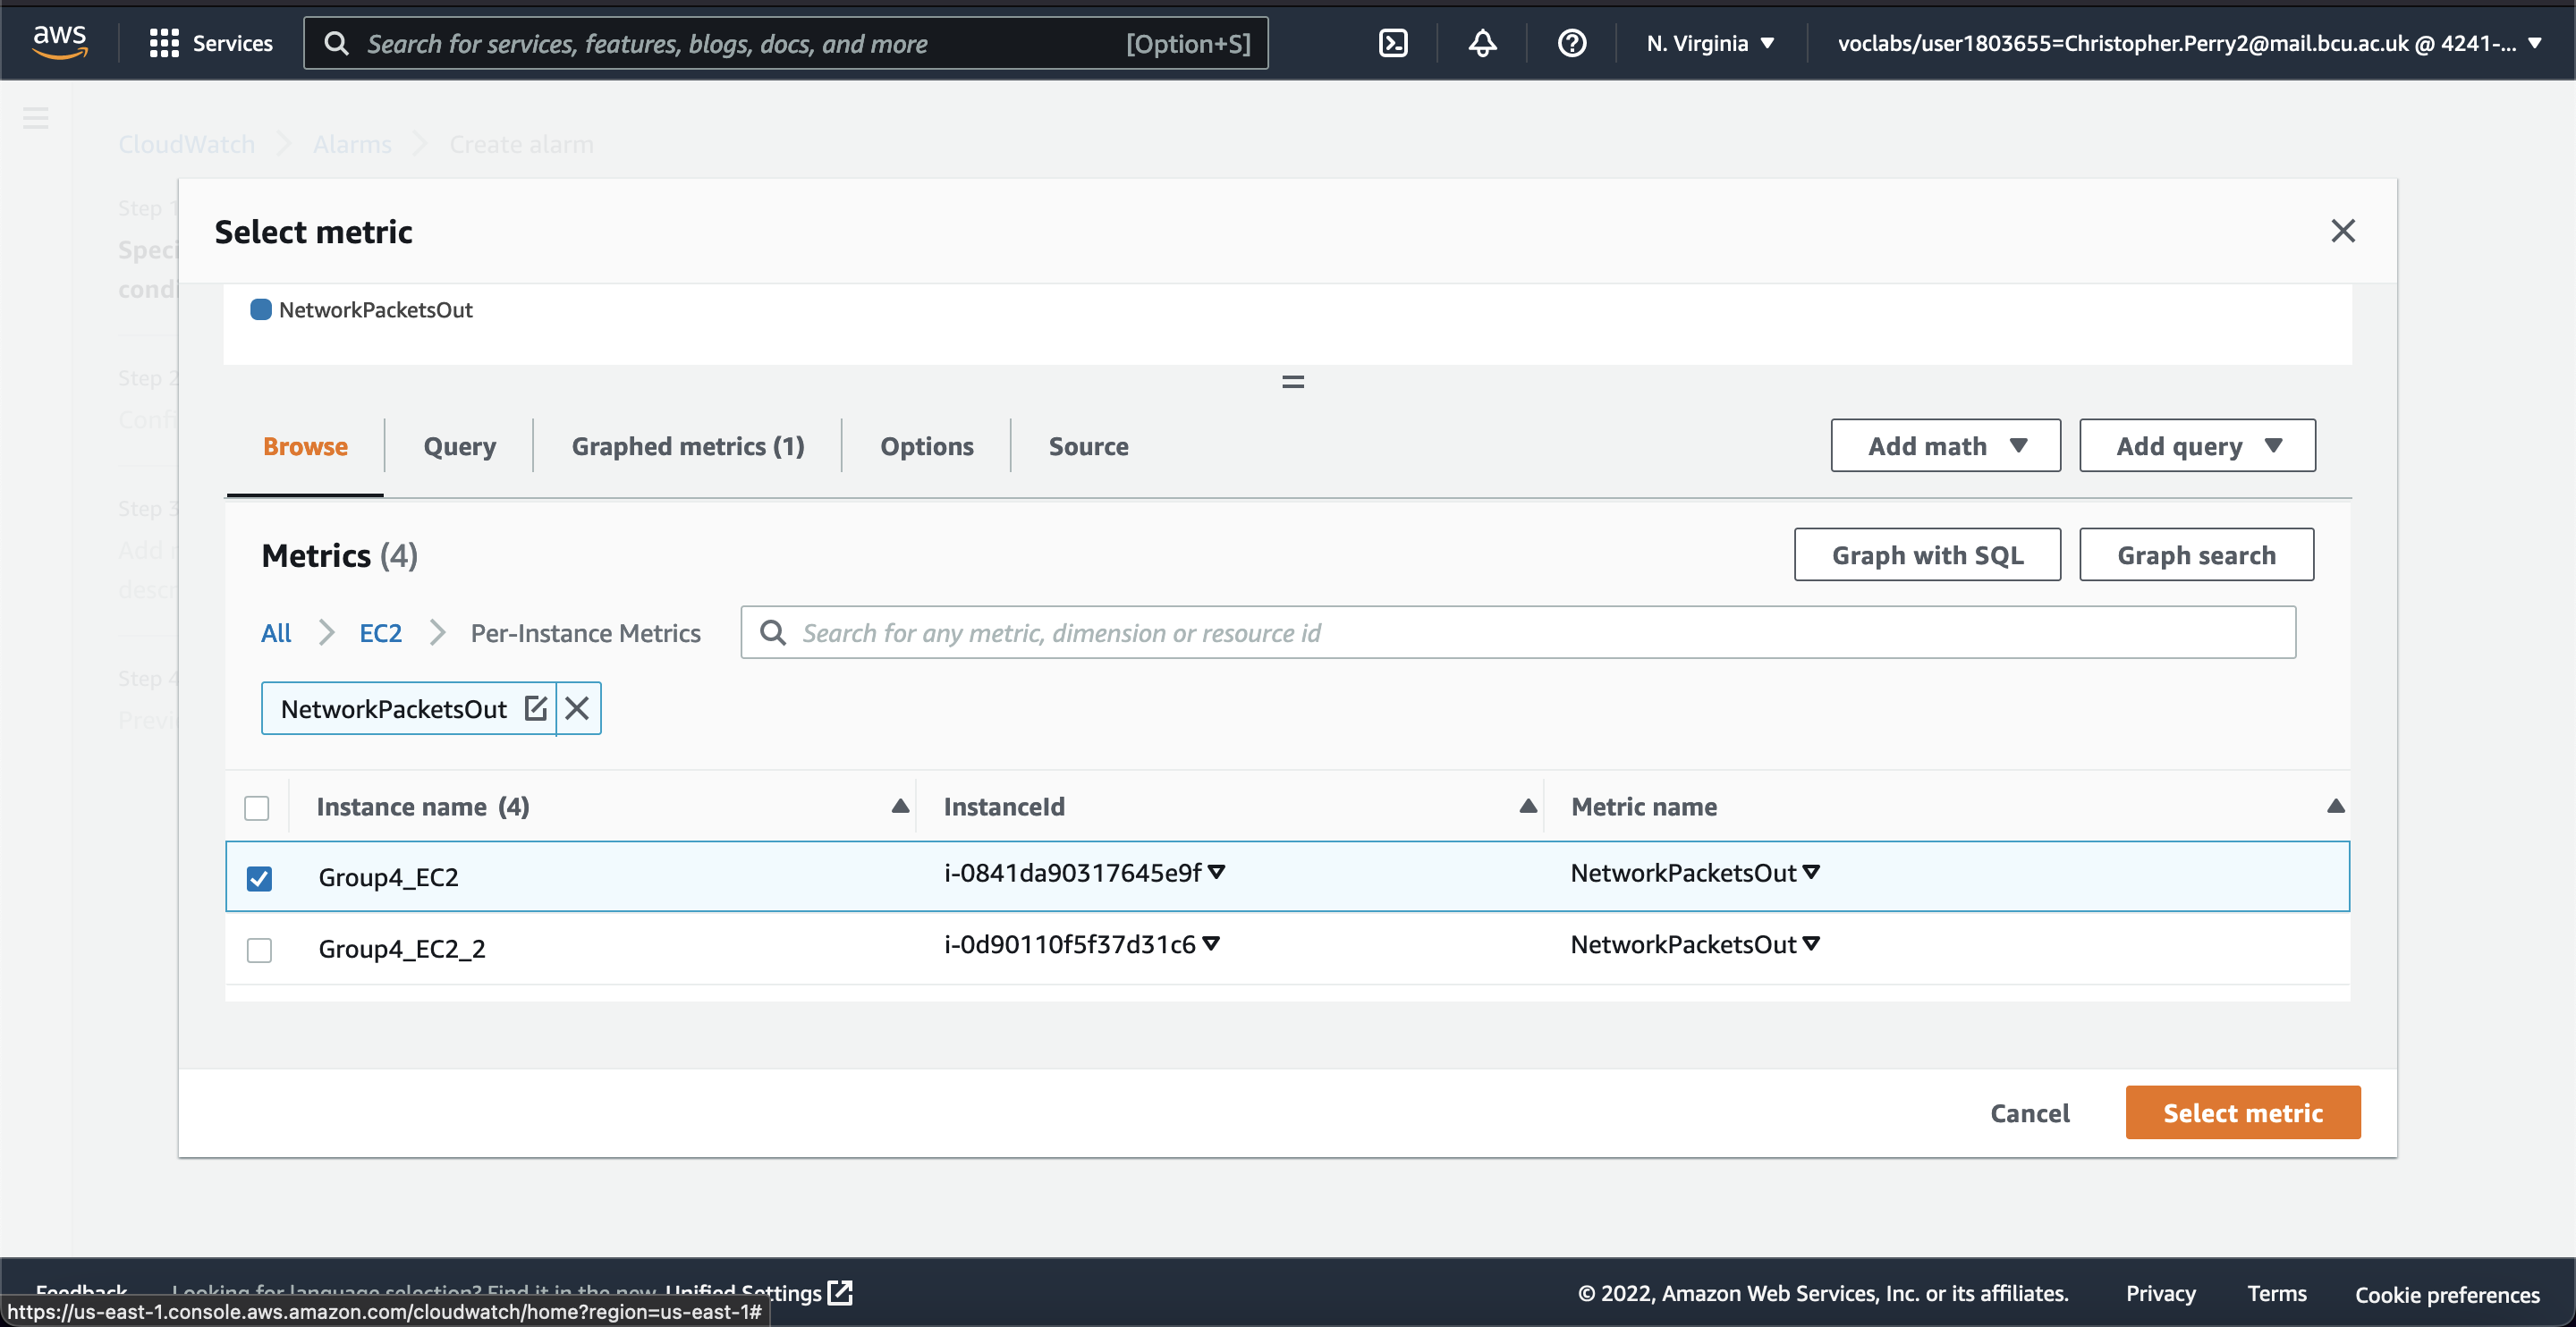
\includegraphics[width=\textwidth]{resources/cloudwatch/cloudwatch-metric-selection}
    \caption{Selection of CloudWatch metric for EC2 instance.}
    \label{fig:cloudwatch-metrics}
\end{figure}

The metric will be configured to alarm in the event that there is less than 5 packets of data sent per day from the
instance.
As the instance currently outputs nearly, 30,000 packets per day, this will be useful to check if the web app has failed.

\begin{figure}[!htbp]
    \centering
    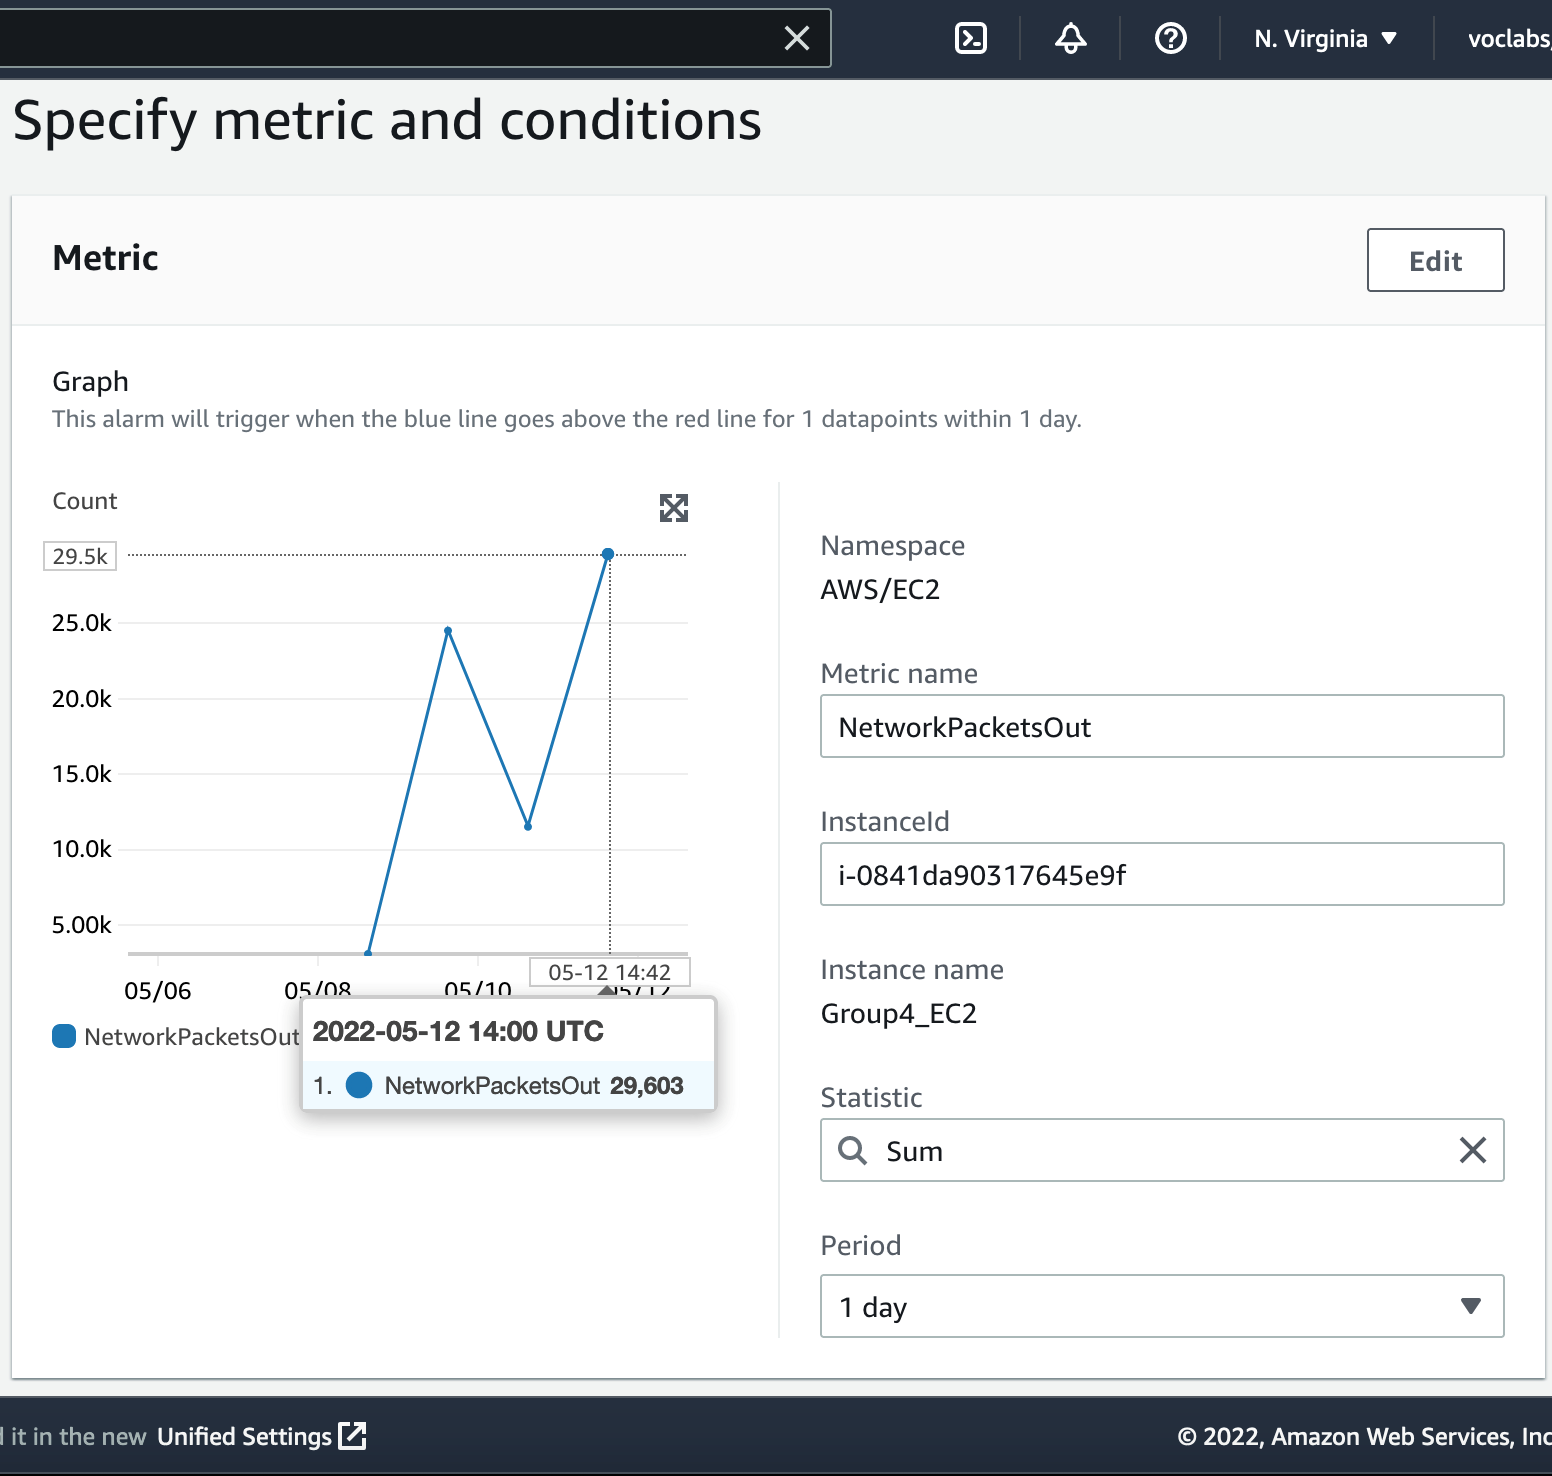
\includegraphics[width=\textwidth]{resources/cloudwatch/cloudwatch-metric-config-1}
    \caption{Configuration of NetworkPacketsOut Metric.}
    \label{fig:cloudwatch-metrics-config-1}
\end{figure}

\begin{figure}[!htbp]
    \centering
    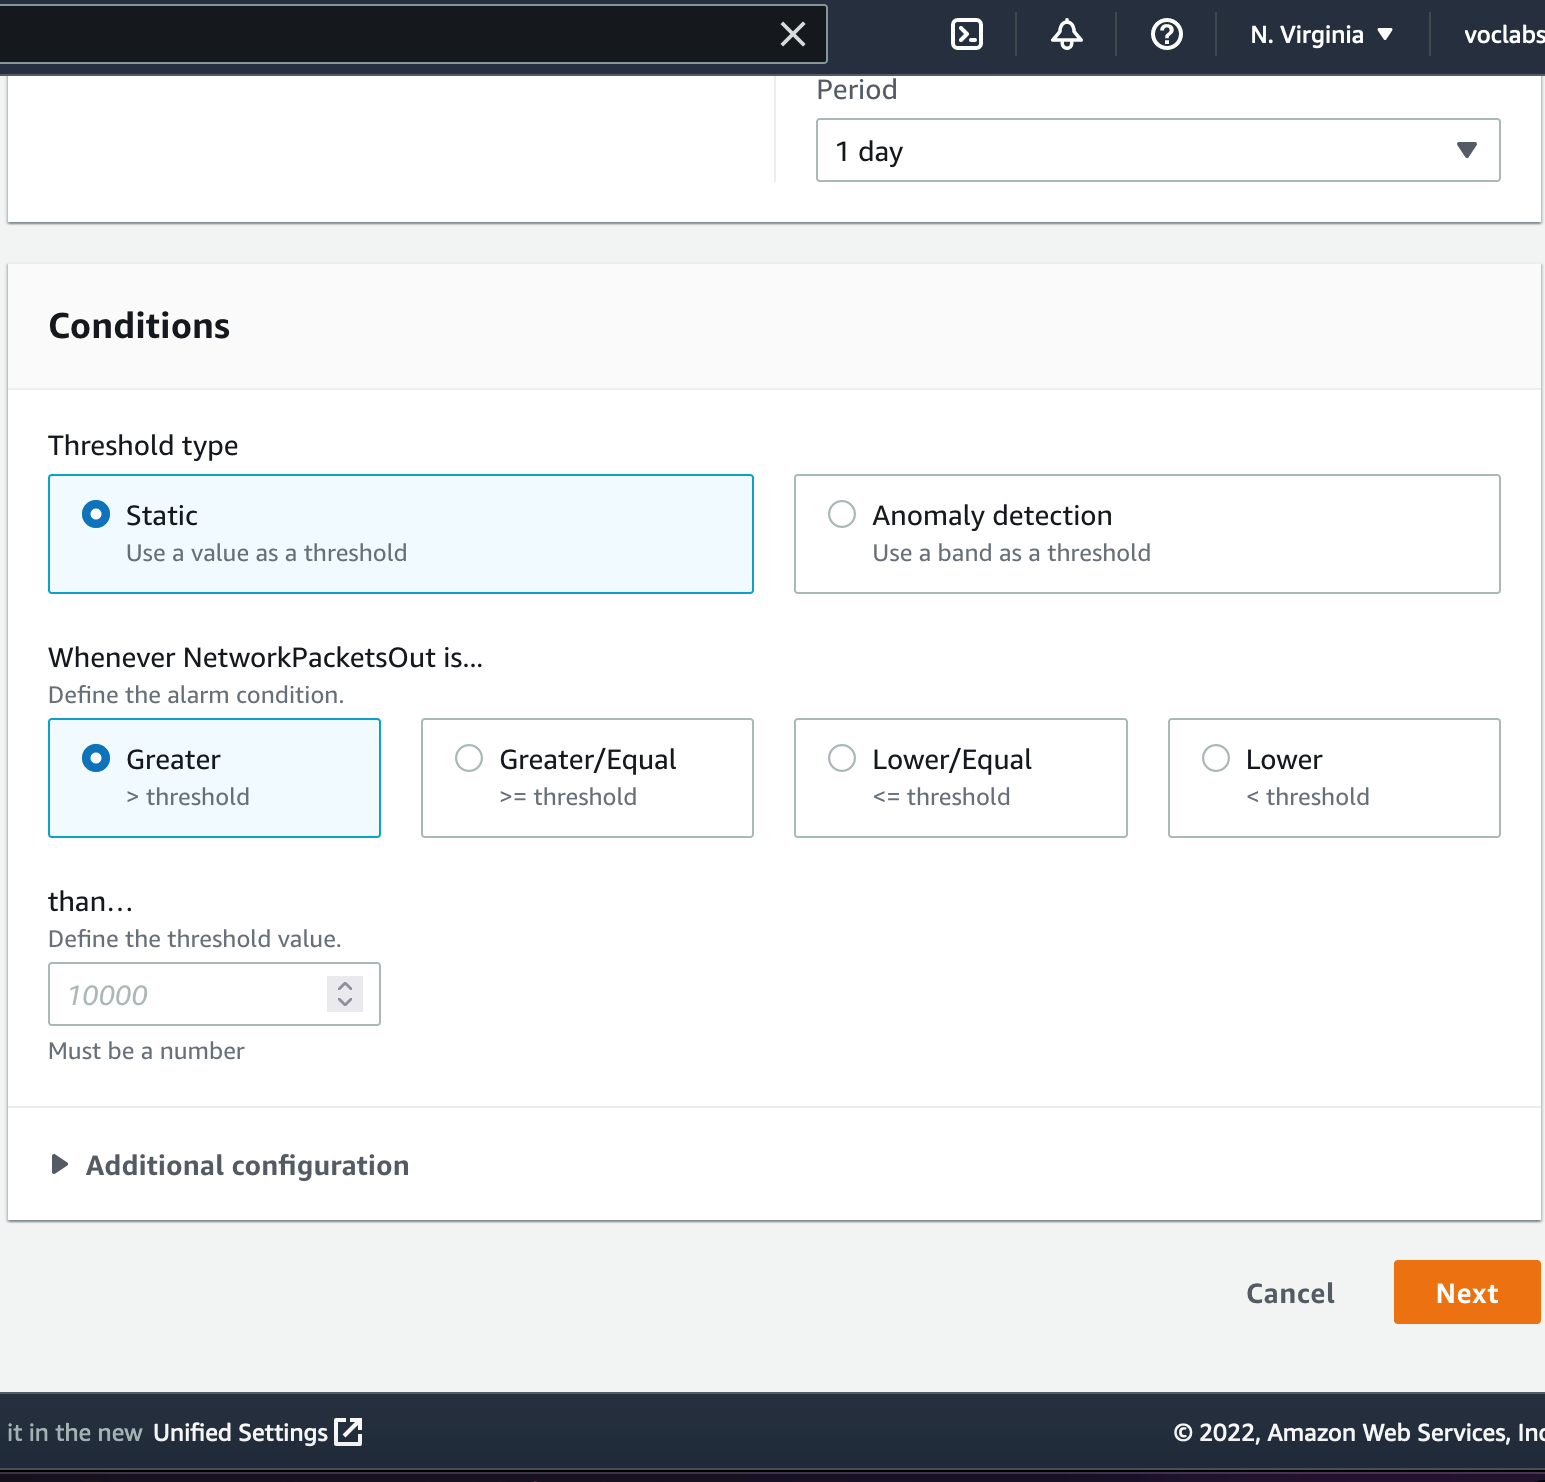
\includegraphics[width=\textwidth]{resources/cloudwatch/cloudwatch-metric-config-2}
    \caption{Configuration of NetworkPacketsOut Metric.}
    \label{fig:cloudwatch-metric-config-2}
\end{figure}

Figures~\ref{fig:cloudwatch-metrics-config-1} and~\ref{fig:cloudwatch-metric-config-2} detail the alarm being set so that
when the sum of packets sent is less than 5 per day, the alarm will activate.

In addition to the initial configuration of these CloudWatch alarms, SNS topics will also be set up so that every member
of the group will be emailed in the event that the alarms activate.
Figure~\ref{fig:cloudwatch-sns-topic} details this process.

\begin{figure}[!htbp]
    \centering
    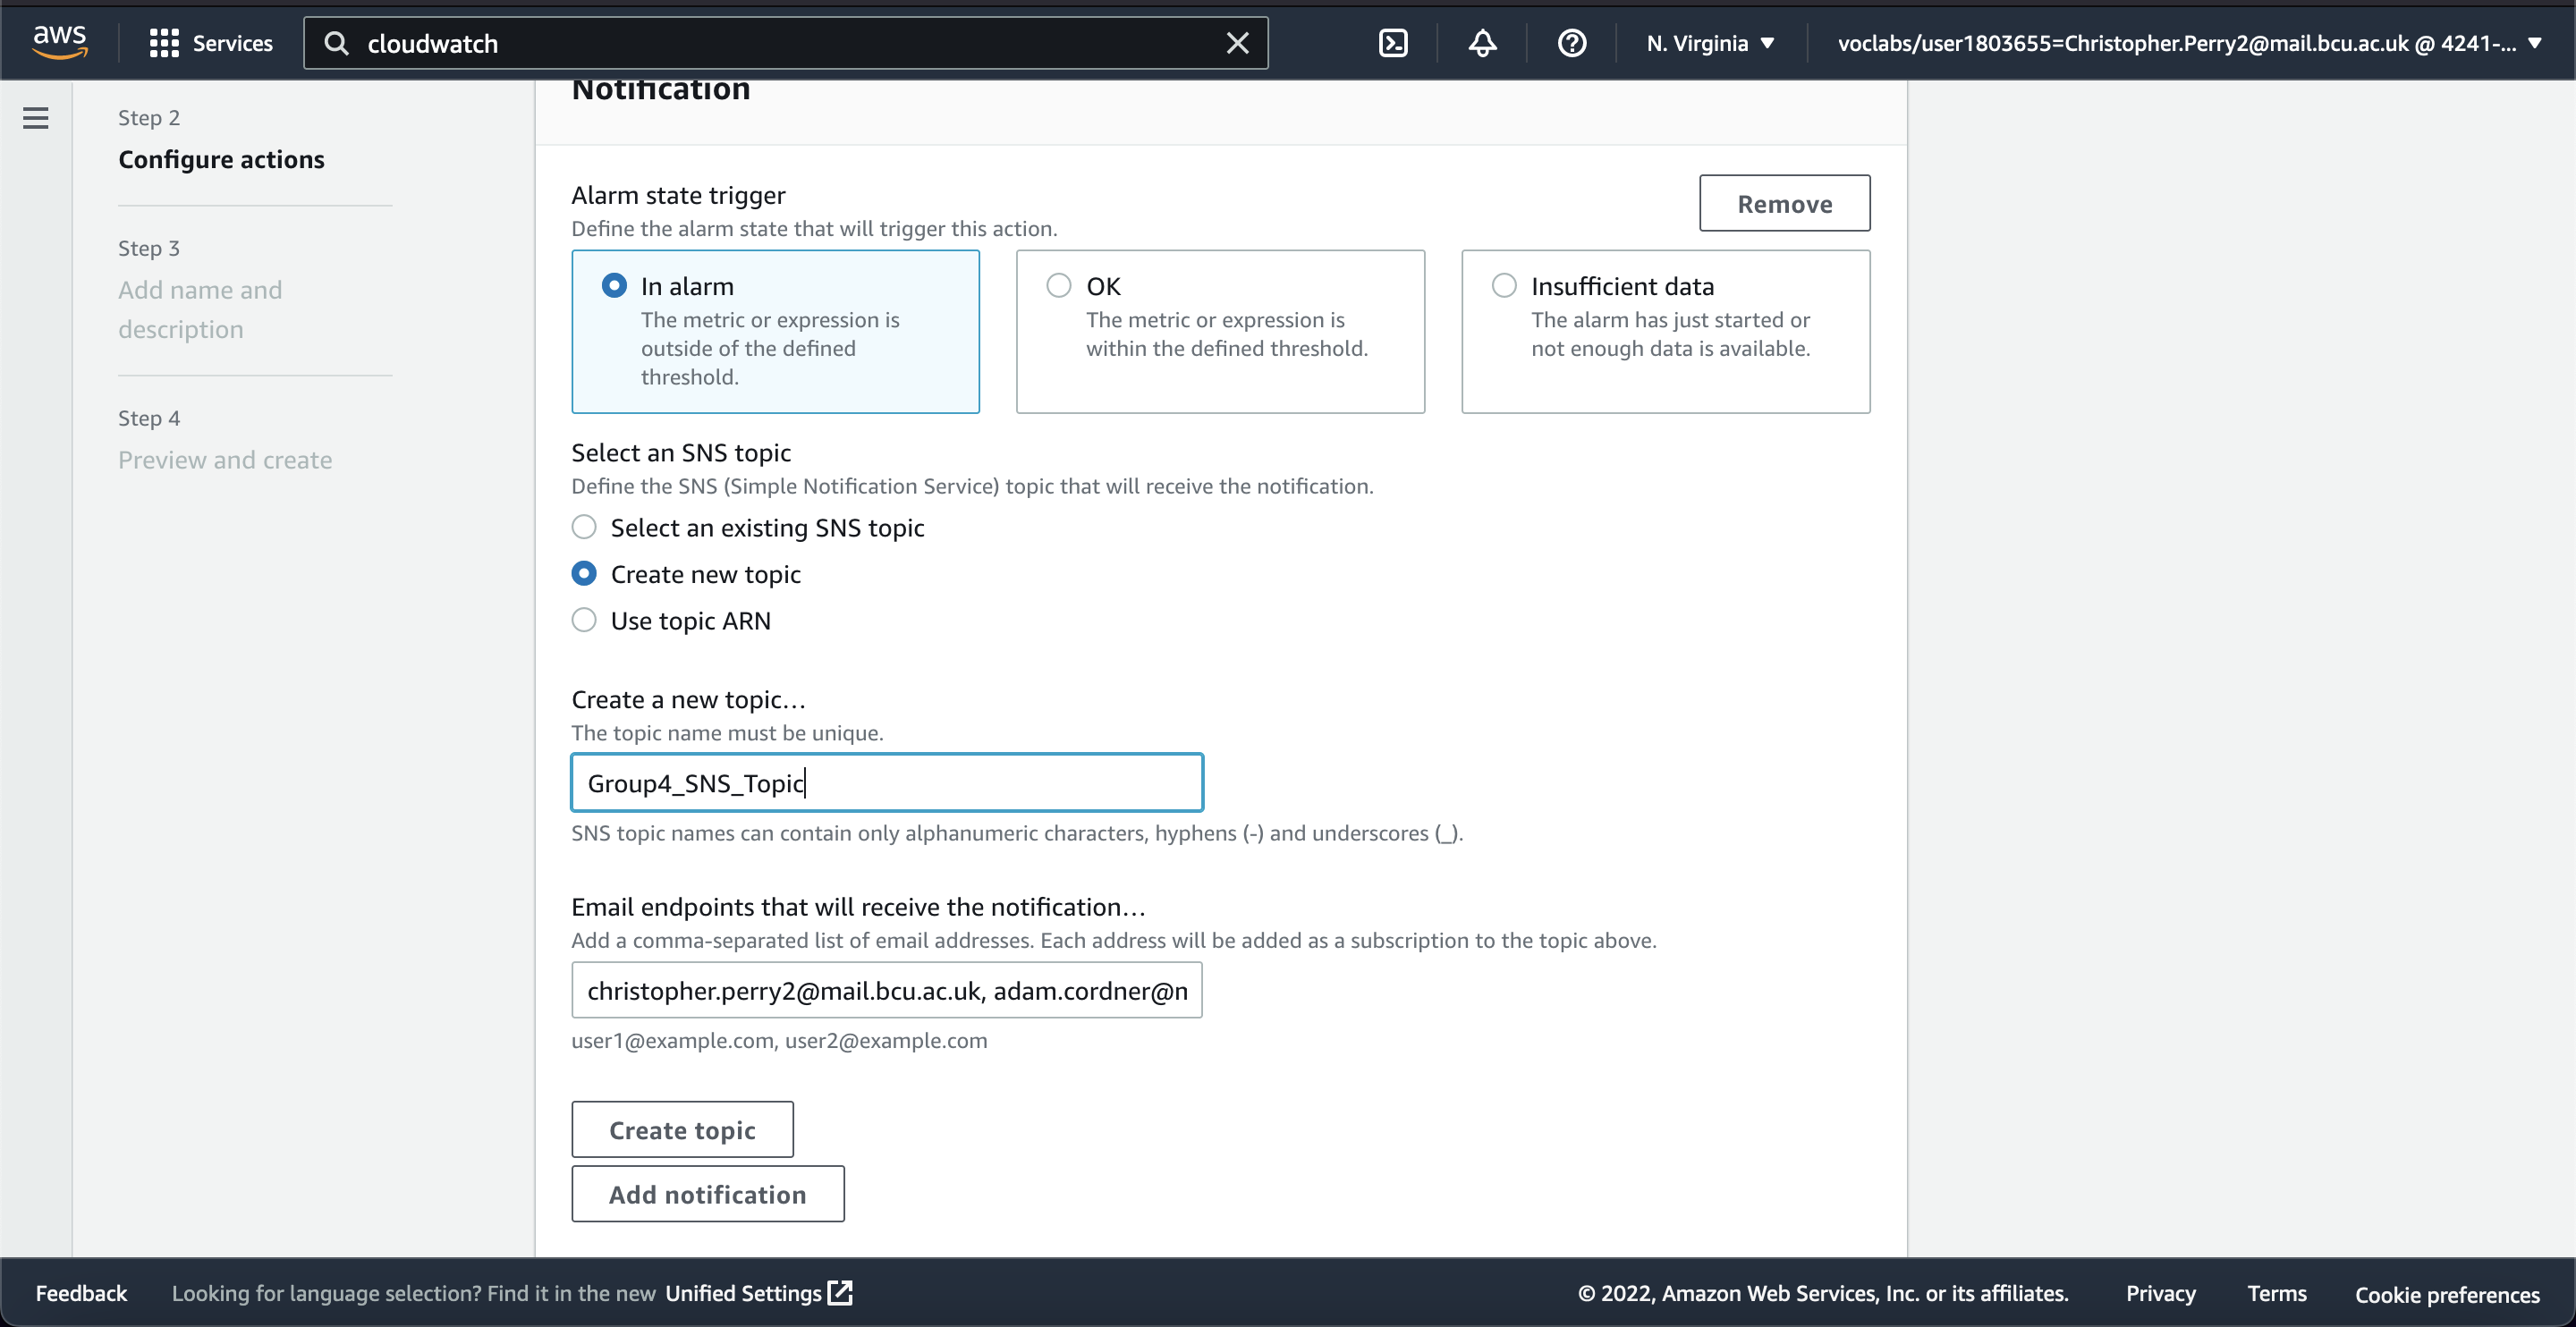
\includegraphics[width=\textwidth]{resources/cloudwatch/cloudwatch-sns-topic}
    \caption{Configuration of SNS Topic for email alerts on alarm activation.}
    \label{fig:cloudwatch-sns-topic}
\end{figure}

An email was then sent to all group members upon completion of this form, and the SNS topic was subsequently subscribed
to, as shown in Figures~\ref{fig:cloudwatch-sns-email} and~\ref{fig:cloudwatch-sns-success}.

\begin{figure}[!htbp]
    \centering
    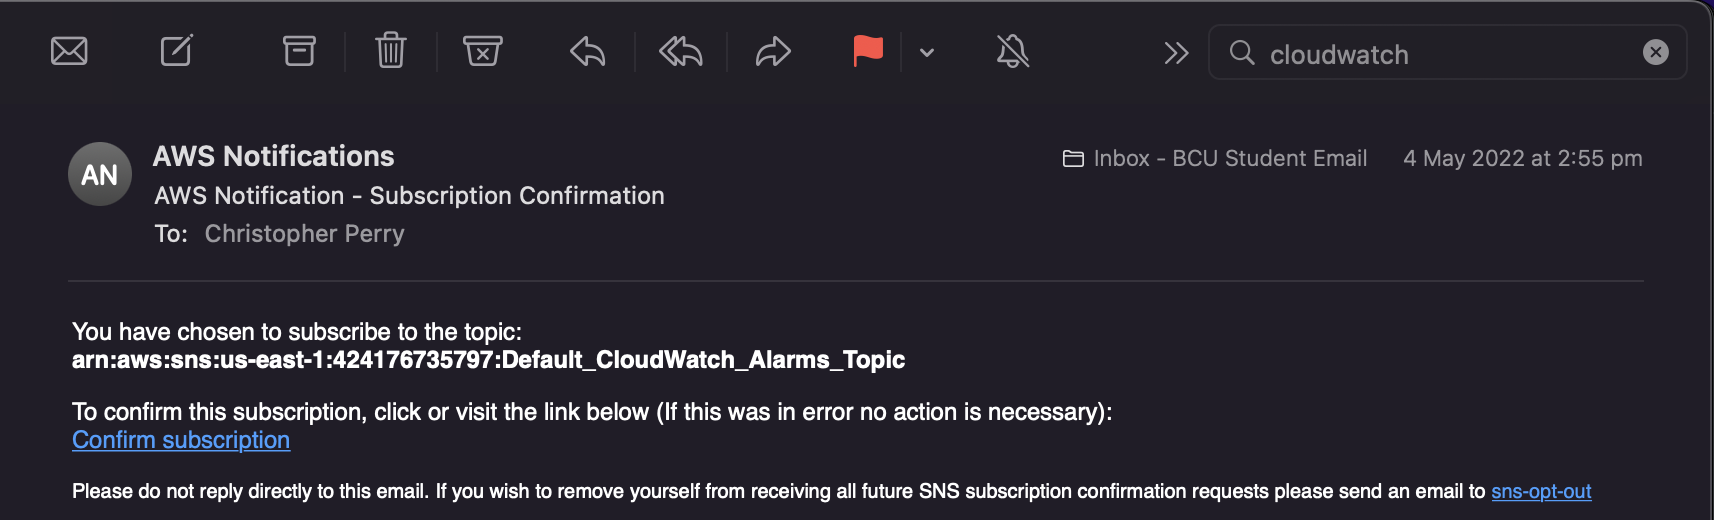
\includegraphics[width=\textwidth]{resources/cloudwatch/cloudwatch-email}
    \caption{CloudWatch SNS Topic Email.}
    \label{fig:cloudwatch-sns-email}
\end{figure}

\begin{figure}[!htbp]
    \centering
    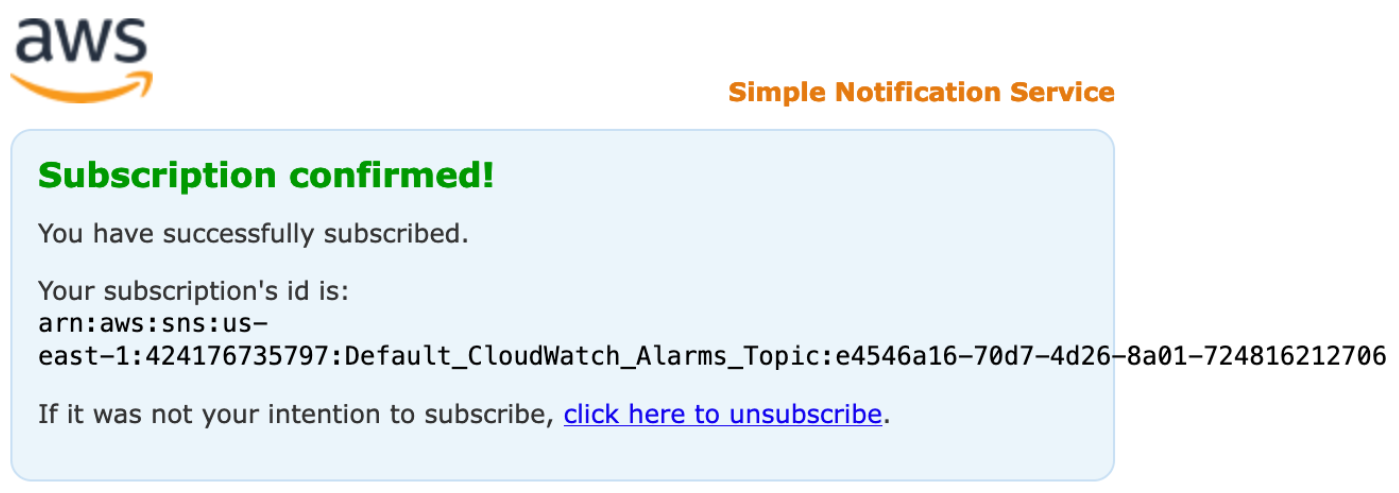
\includegraphics[width=\textwidth]{resources/cloudwatch/cloudwatch-alarm-success}
    \caption{Successful subscription to SNS topic.}
    \label{fig:cloudwatch-sns-success}
\end{figure}

The EC2 instance has also been configured to restart when this alarm activates.
This is done by automatically re-running the scripts used to start the web app on the instance starting up again.

This process can be seen in Figure~\ref{fig:cloudwatch-ec2-actions}.

\begin{figure}[!htbp]
    \centering
    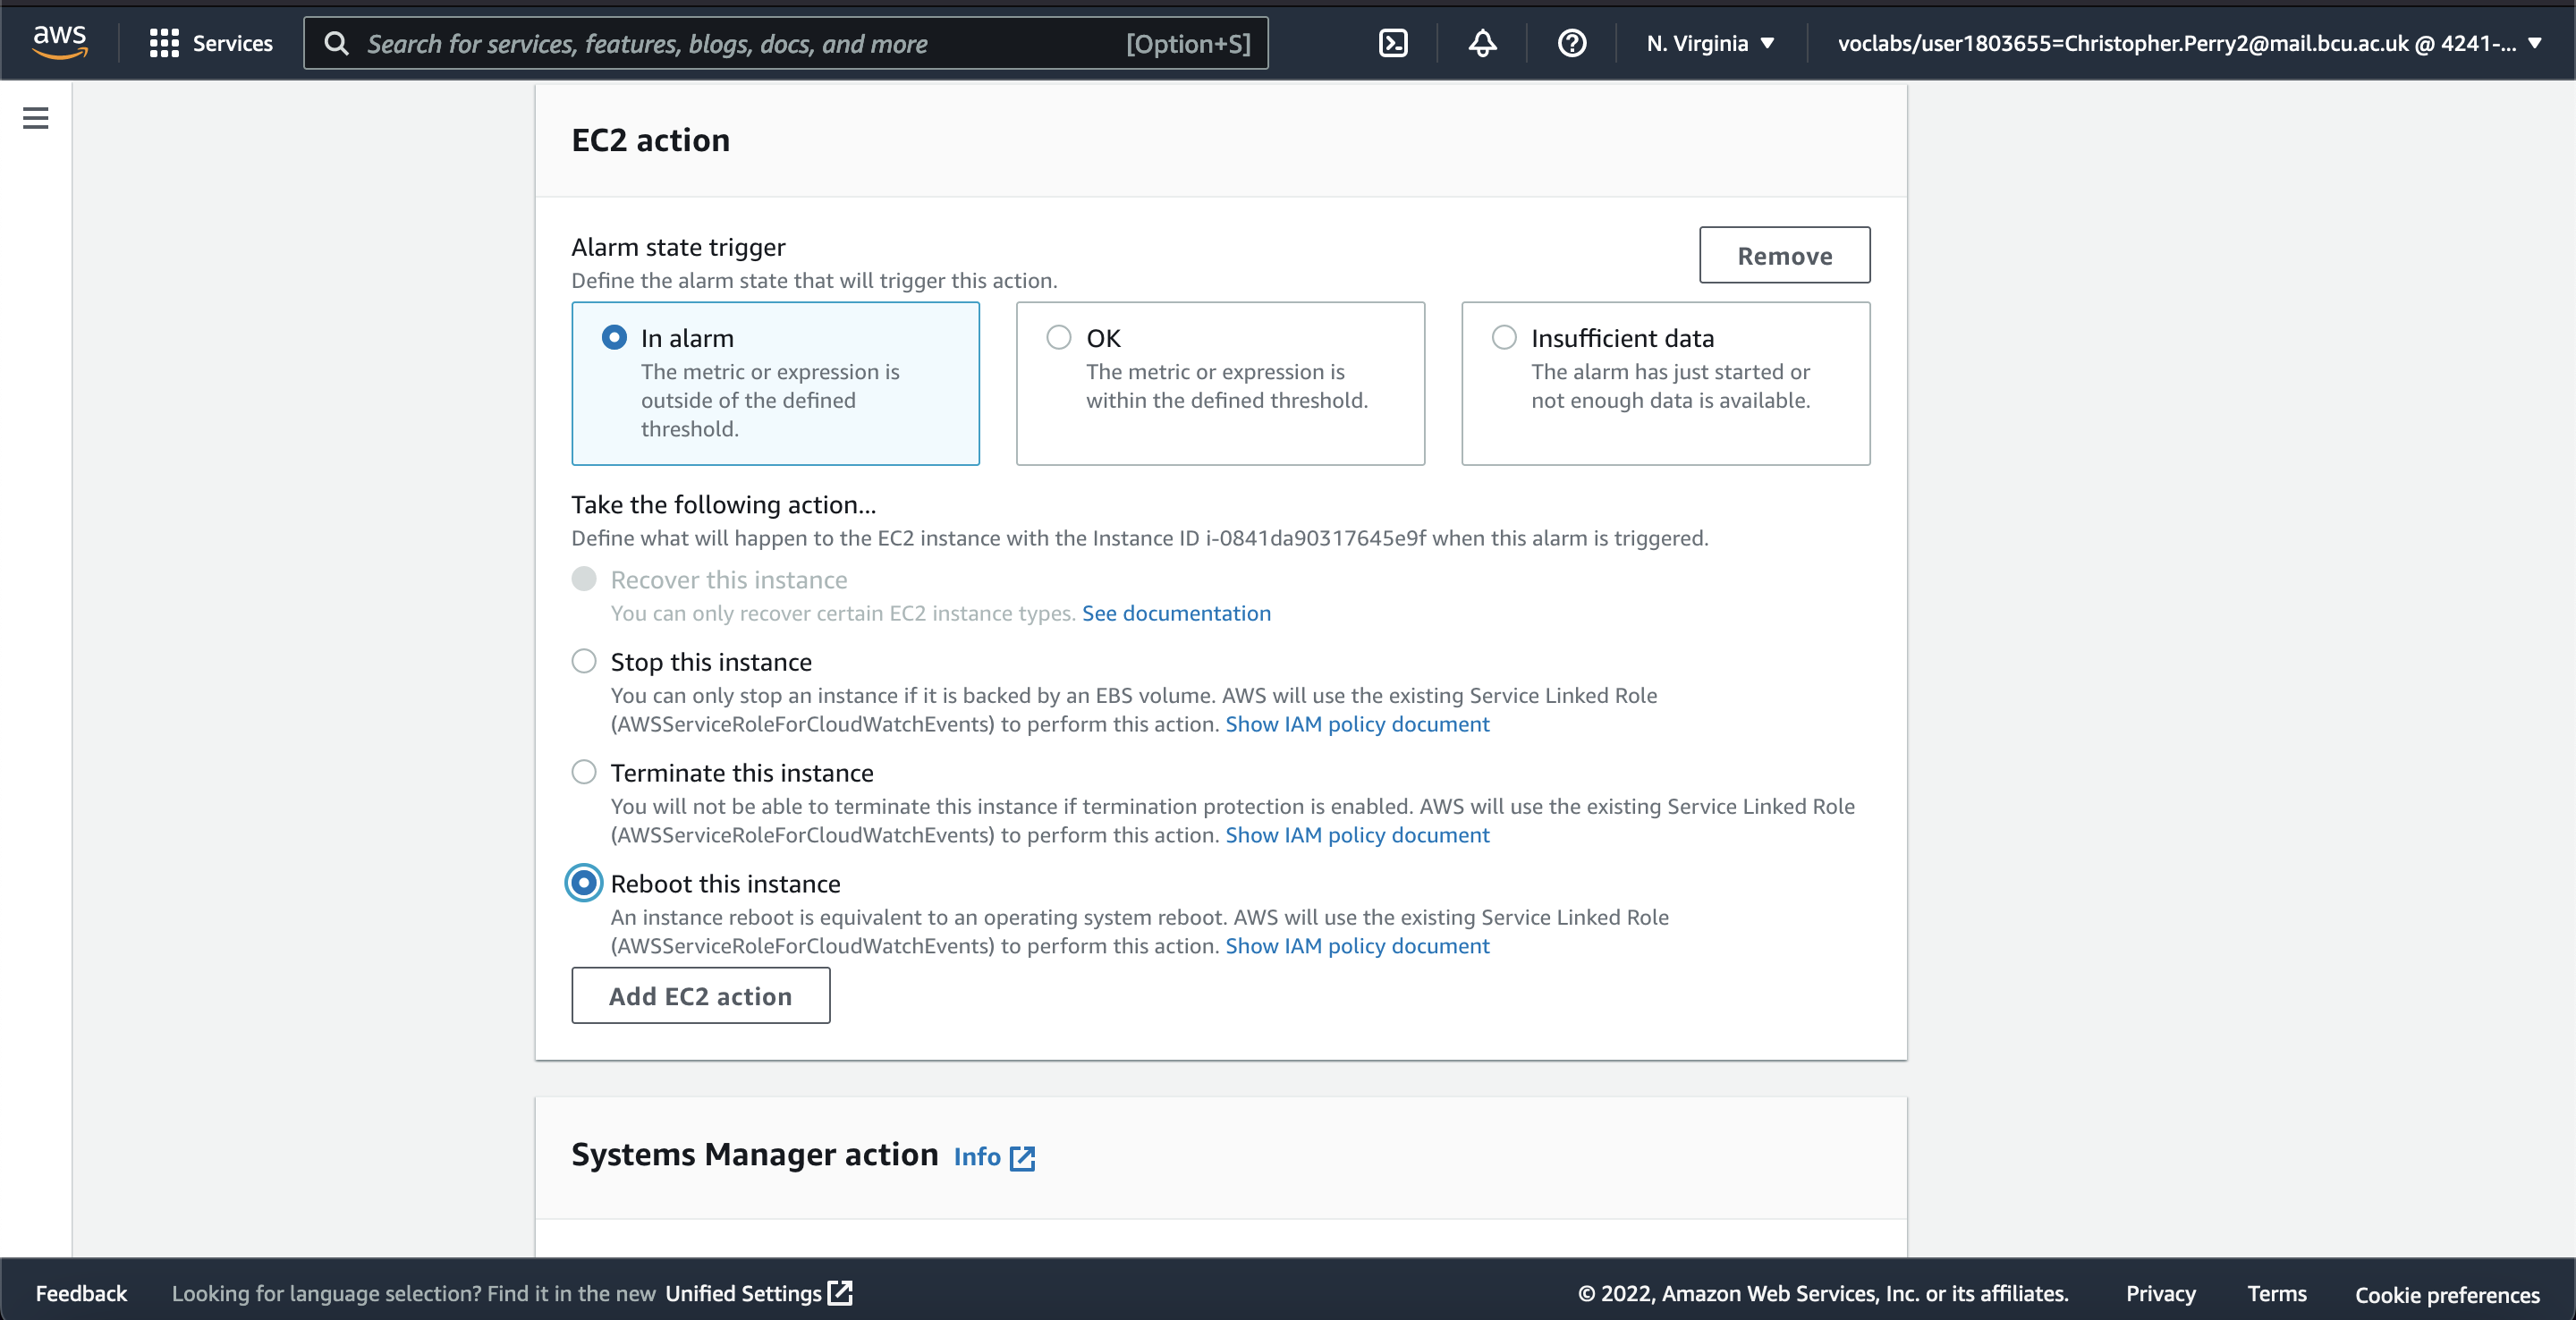
\includegraphics[width=\textwidth]{resources/cloudwatch/cloudwatch-ec2-actions}
    \caption{Configuration for EC2 instance to reboot on alarm activation.}
    \label{fig:cloudwatch-ec2-actions}
\end{figure}

A brief description of the CloudWatch alarm is then added.
This can be seen in Figure~\ref{fig:cloudwatch-description}.

\begin{figure}[!htbp]
    \centering
    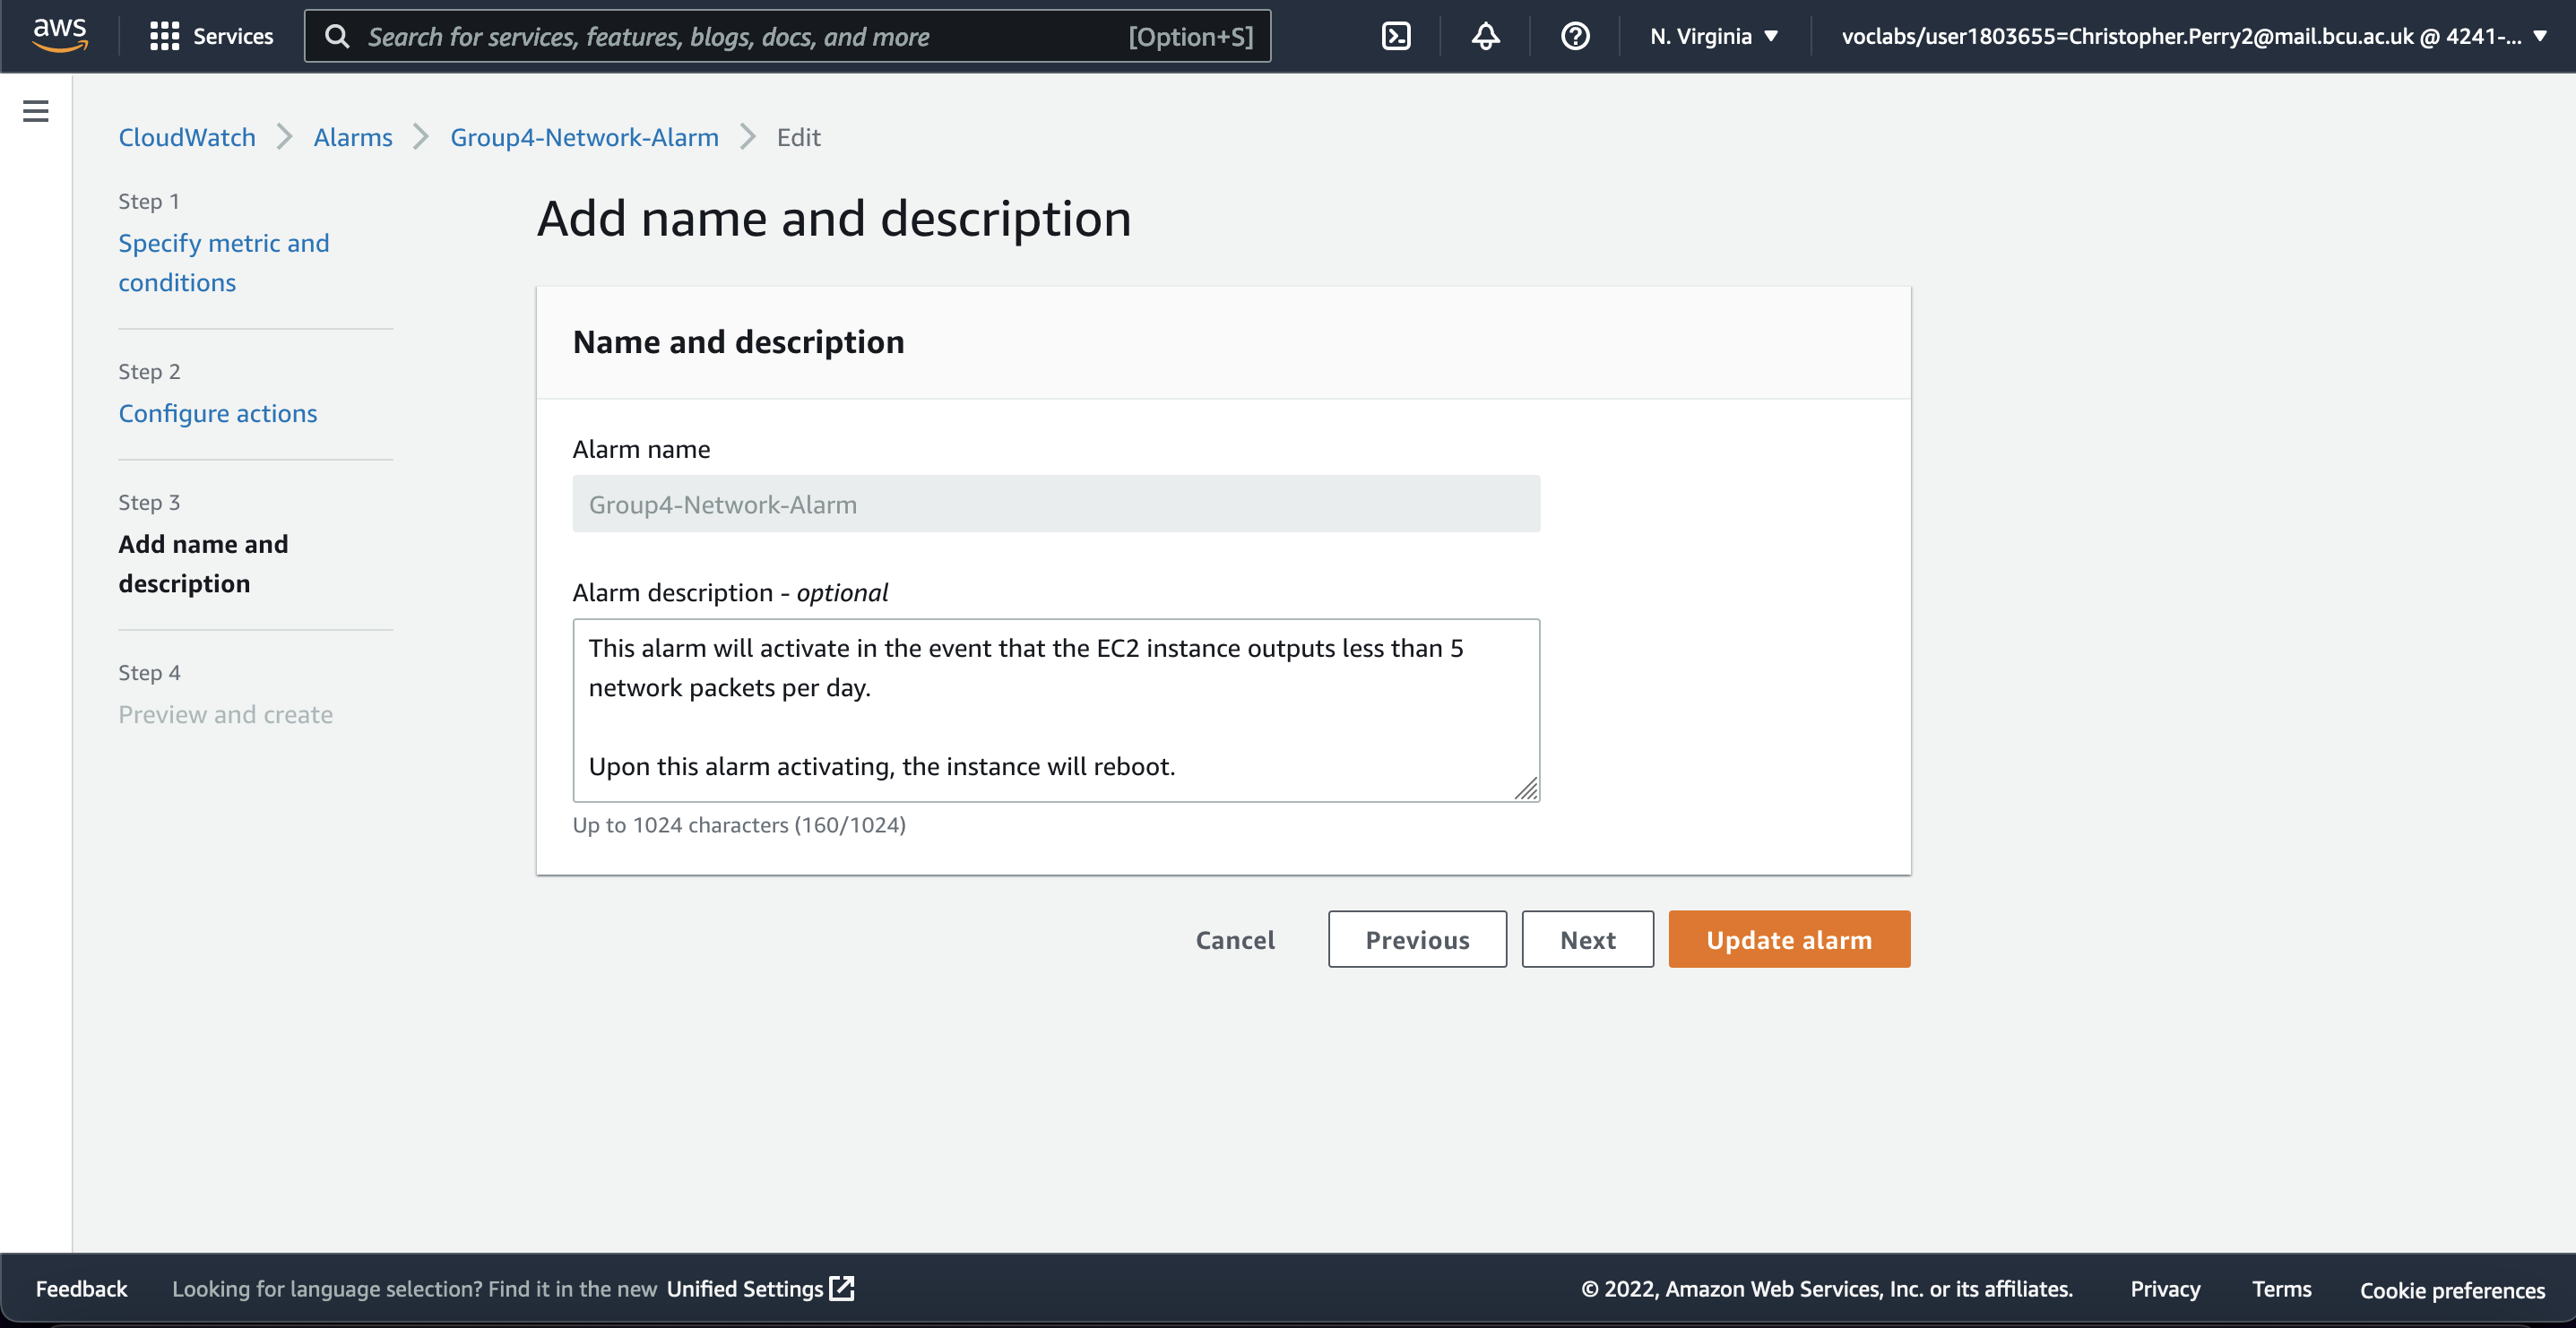
\includegraphics[width=\textwidth]{resources/cloudwatch/cloudwatch-description}
    \caption{CloudWatch alarm description.}
    \label{fig:cloudwatch-description}
\end{figure}

The alarm has now been set up, and can be seen in the CloudWatch Management Dashboard in Figure~\ref{fig:cloudwatch-network-alarm}.

\begin{figure}[!htbp]
    \centering
    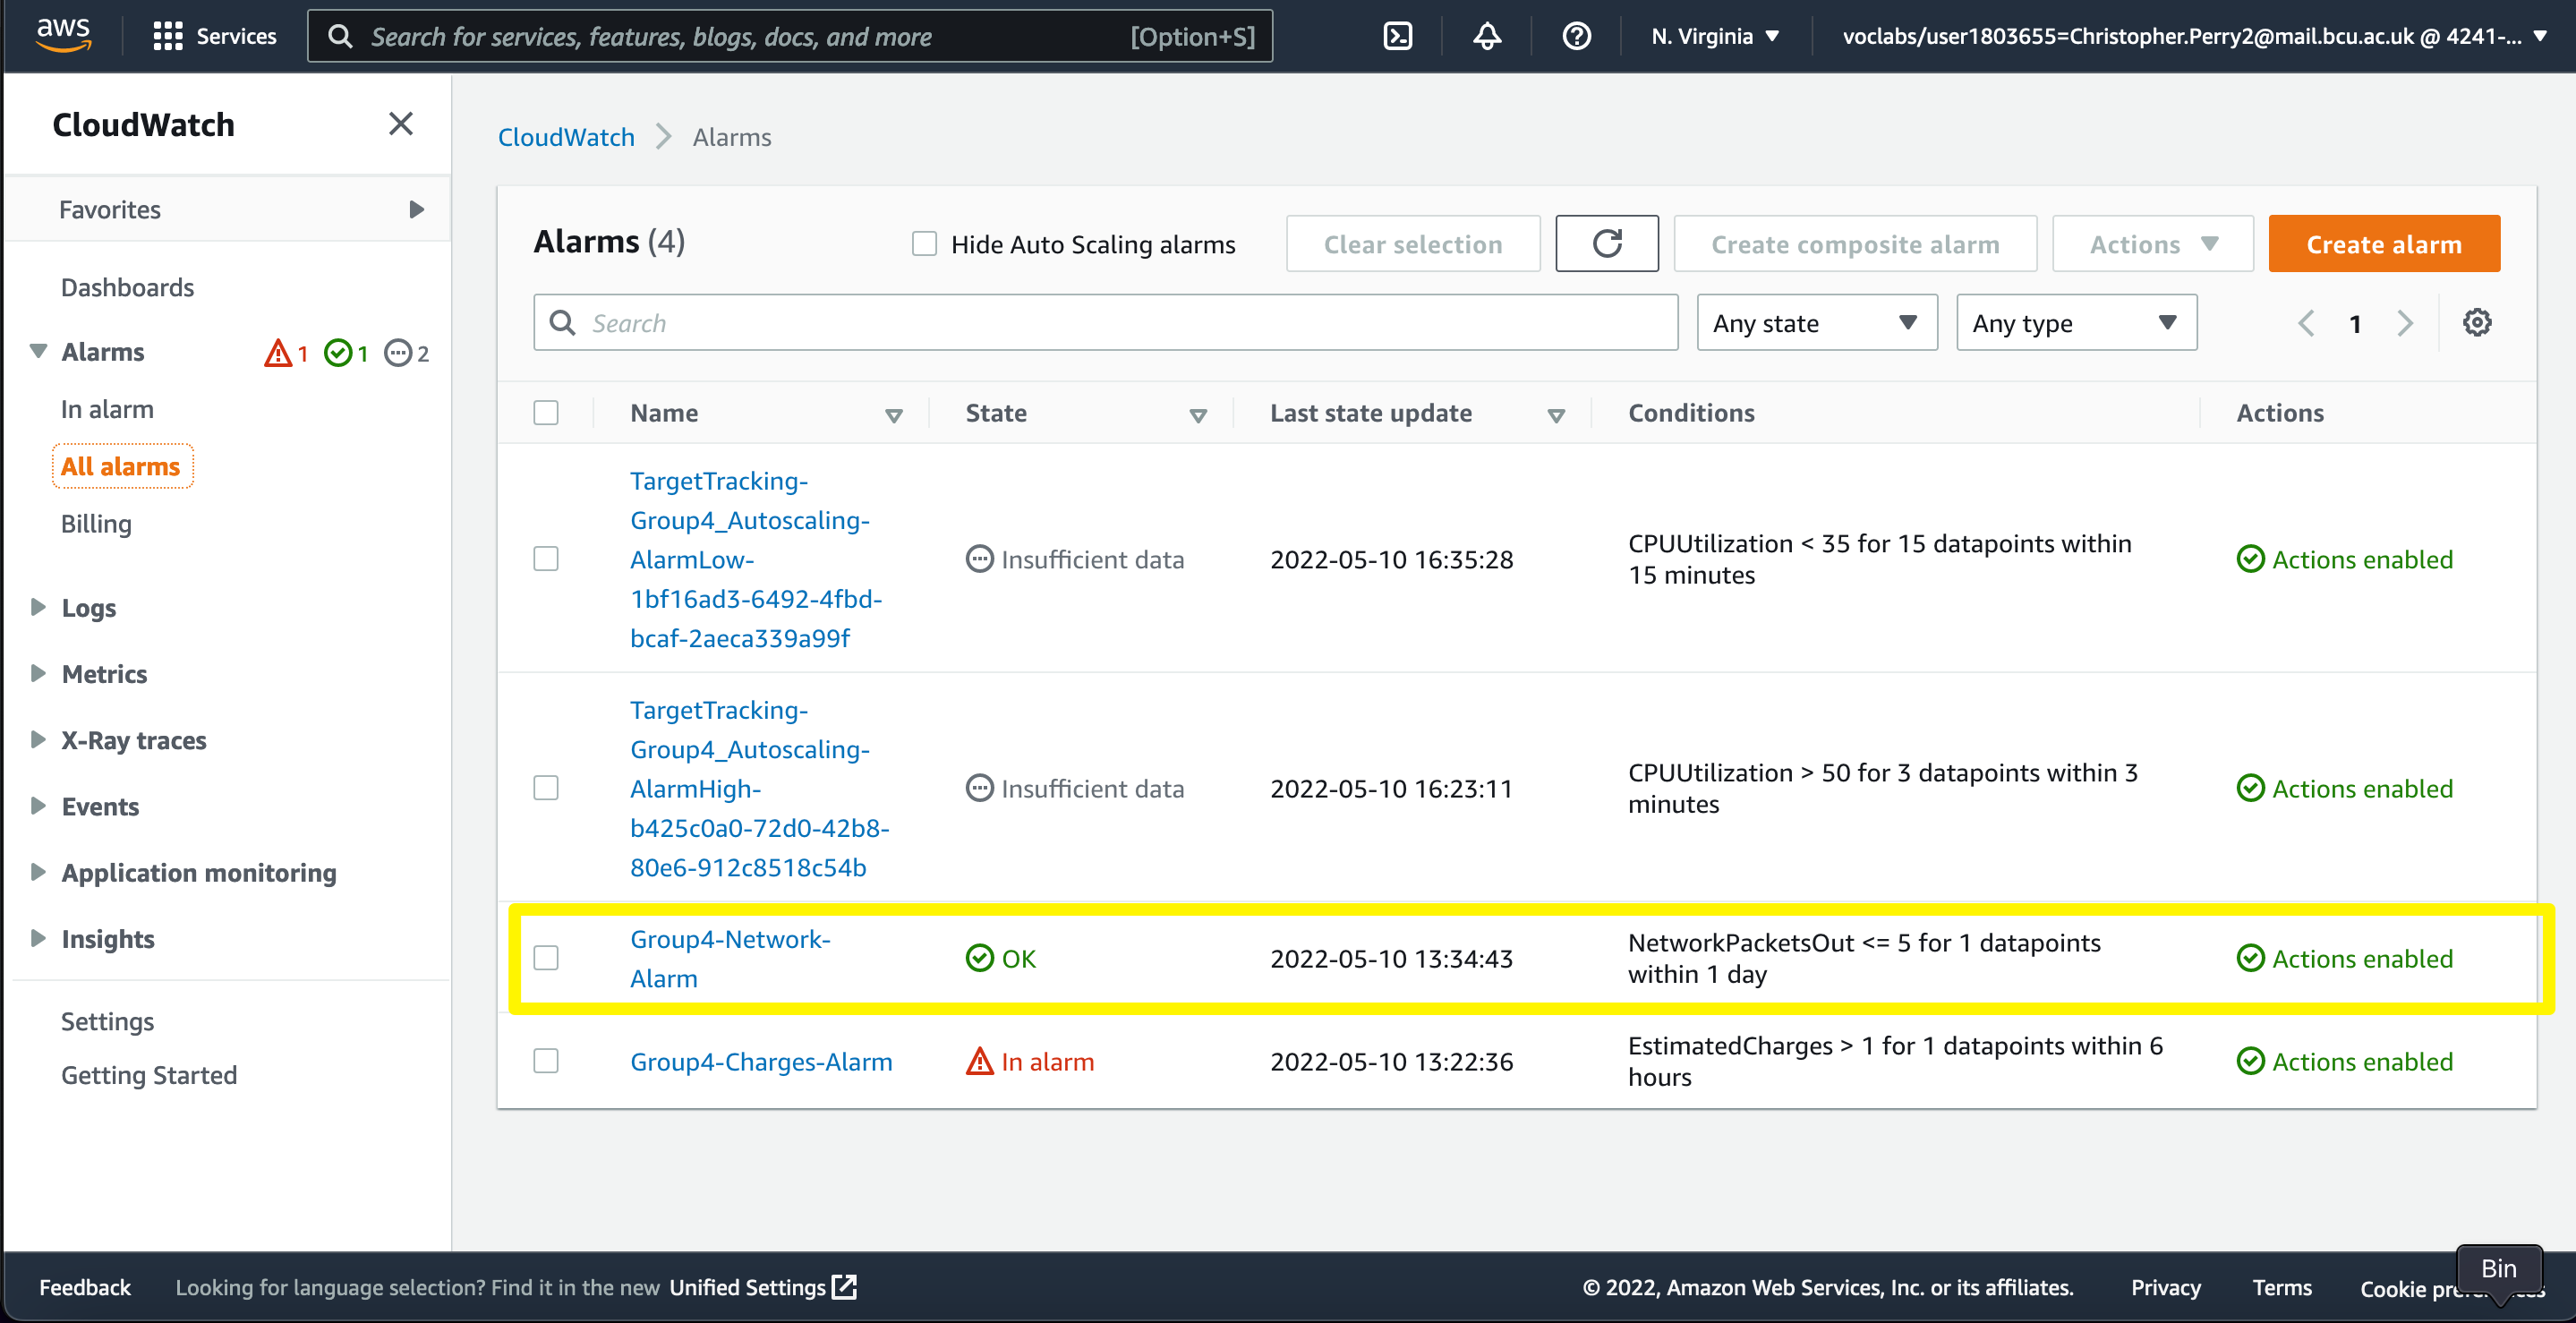
\includegraphics[width=\textwidth]{resources/cloudwatch/cloudwatch-network-alarm-complete}
    \caption{CloudWatch network alarm in dashboard.}
    \label{fig:cloudwatch-network-alarm}
\end{figure}







